\subsection{Outras customizações realizadas no algoritmo}
\label{outrasVersoes}

O \gls{MEC} em sua implementação para classificação de candidatos do \gls{SISU} para o primeiro semestre de 2018, acabou por adotar em seu sistema um entendimento distinto sobre questões de arredondamento de vagas em contra-mão do que era descrito na portaria normativa nº 18/2012/MEC:

\begin{citacao}
Art. 11 - Sempre que a aplicação dos percentuais para a apuração da reserva de vagas de que trata o art. 10 implicar resultados com decimais, será adotado, em cada etapa do cálculo, o número inteiro imediatamente superior \cite{portarianr9}.
\end{citacao}

\begin{figure}[h!]
\centering

\caption{\textmd{Solicitação de correções para processos SISU}}
\label{fig:seres}
\fcolorbox{gray}{white}{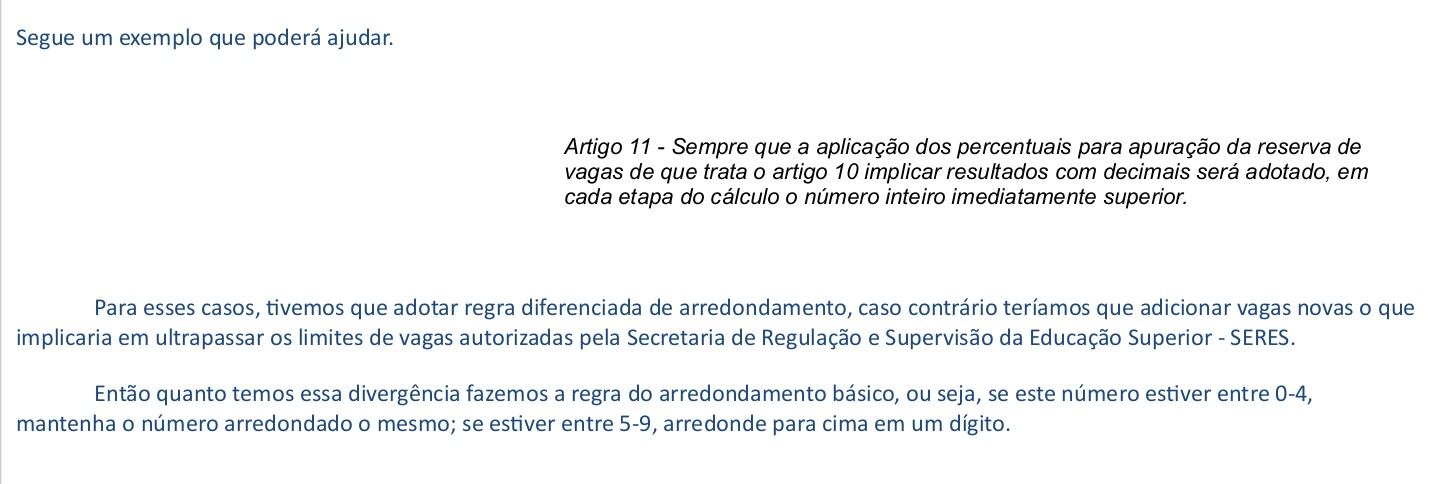
\includegraphics[width=\textwidth]{chapters/sistemaingresso_versoes/imagens/seres.jpg}}

\par\medskip\textbf{Fonte:} Servidor de e-mails do IFSC \par\medskip

\end{figure}



\newpage
A área demandante do \gls{IFSC} em consulta com a \gls{SERES} recebeu o retorno de que tiveram que adotar regra diferenciada de arredondamento do exigido em lei, por questões de limitação de vagas (Figura \ref{fig:seres}), algumas categorias não poderiam ser atendidas na época, obrigando que o sistema de ingresso do \gls{IFSC} fosse ajustado para a modalidade de processos do tipo \gls{SISU}, principalmente para chamada de vagas posteriores à classificação gerada pelo \gls{SISU}.

Nesse contexto, a equipe de desenvolvimento da \gls{DTIC} precisou fazer correções no algoritmo de classificação para considerar o arredondamento diferenciado. Com isso, inseriu novas configurações em banco de dados para o cálculo condicionando à modalidade do processo, mantendo a compatibilidade com processos que seguem a forma de arredondamento prevista em lei.

A exemplo do desenvolvimento necessário para essa correção de arredondamento, o sistema de controle de versão indica como 8 (oito) arquivos PHP modificados, sendo 69 linhas adicionadas e 44 linhas removidas, além da necessidade de inclusão de 2 (dois) novos campos na tabela de configurações do sistema de cotas (Figura \ref{fig:versaosisu}).

\begin{figure}[h!]
\centering

\caption{\textmd{Controle de versão para correções SISU}}
\label{fig:versaosisu}
\fcolorbox{gray}{white}{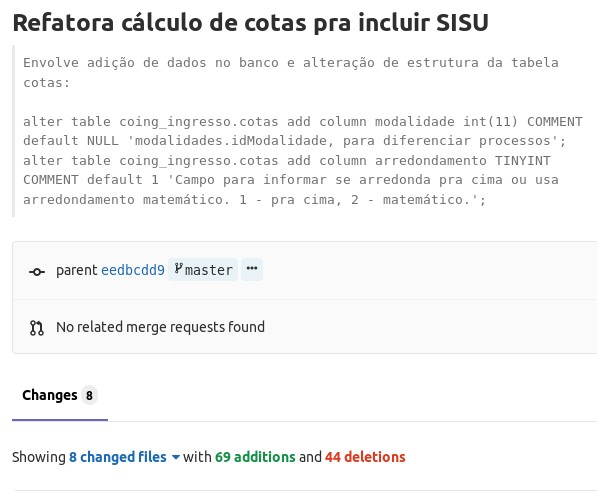
\includegraphics[width=\textwidth]{chapters/sistemaingresso_versoes/imagens/versaosisu.jpg}}

%\par\medskip\textbf{Fonte:} \cite{sitemec} \par\medskip

\end{figure}



\newpage
Essas foram as maiores alterações levantadas no sistema de controle de versões do \gls{IFSC}, no entanto, pode-se observar na Figura \ref{fig:trello}, que foram criadas várias demandas na ferramenta \textit{Trello} (utilizada para gerenciamento do desenvolvimento interno), assim como vários chamados de cunho corretivo.  

%\begin{figure}[ht!]
\centering

\caption{\textmd{Chamados sobre cotas no sistema de ingresso}}
\label{fig:chamados}
\fcolorbox{gray}{white}{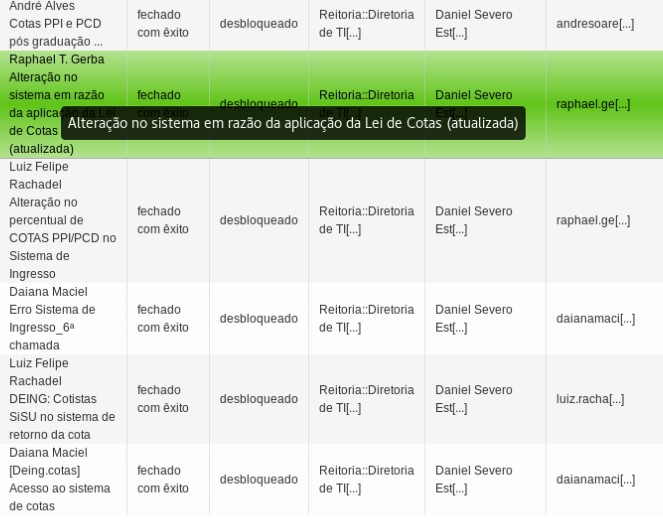
\includegraphics[width=0.7\textwidth]{chapters/sistemaingresso_versoes/imagens/chamados.jpg}}
\par\medskip\textbf{Fonte:} Elaboração do autor \par\medskip

\end{figure}



\begin{figure}[h!]
\centering

\caption{\textmd{Demandas sobre o desenvolvimento de cotas}}
\label{fig:trello}
\fcolorbox{gray}{white}{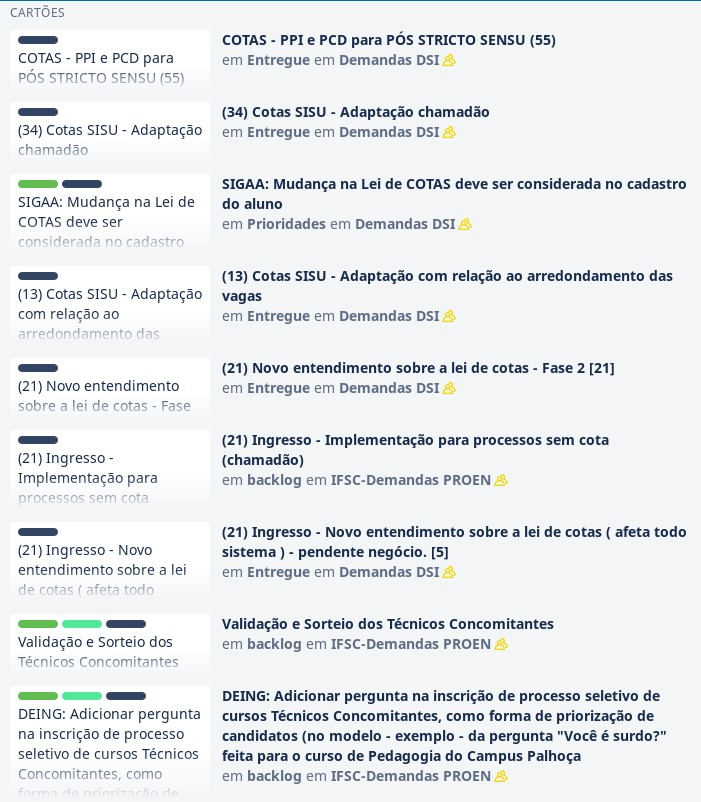
\includegraphics[width=\textwidth]{chapters/sistemaingresso_versoes/imagens/trello.jpg}}

%\par\medskip\textbf{Fonte:} \cite{sitemec} \par\medskip

\end{figure}



\newpage
Na sequência, o Capítulo \ref{metodologia} descreve os procedimentos metodológicos utilizados na pesquisa.






